\documentclass[final]{article}
%%%%%%%%%%%%%%%%%%%%%%%%%%%%%%%%%%%%%%%%%%%%%%%%%%%%%%%%%%%%%
% Lecture Specific Information to Fill Out
%%%%%%%%%%%%%%%%%%%%%%%%%%%%%%%%%%%%%%%%%%%%%%%%%%%%%%%%%%%%%
\newcommand{\LectureTitle}{3D Human Pose Reconstruction from a 2D Monocular Image with Joint Ordering Uncertainty}
%\newcommand{\LectureDate}{\today}
\newcommand{\LectureDate}{December\ 12,\ 2018}
\newcommand{\LatexerName}{Cedric Flamant}
% Author: Cedric Flamant
%%%%%%%%%%%%%%%%%%%%%%%%%%%%%%%%%%%%%%%%%%%%%%%%%%%%%%%%%%%%%

% Change "article" to "report" to get rid of page number on title page
\usepackage{amsmath,amsfonts,amsthm,amssymb}
\usepackage{setspace}
\usepackage{Tabbing}
\usepackage{fancyhdr}
\usepackage{lastpage}
\usepackage{extramarks}
\usepackage{chngpage}
%\usepackage{soul,color}
\usepackage[usenames,dvipsnames]{xcolor}
\usepackage{graphicx,float,wrapfig}
\usepackage{afterpage}
\usepackage{abstract}
\usepackage{siunitx}
\usepackage{mdframed}
\usepackage{physics}
\usepackage{tikz}
\usepackage{mathdots}
\usepackage{mathrsfs}
\usepackage{tabto}
\usepackage{slashed}
\usepackage{enumerate}
\usepackage{tensor}
\usepackage{slashed}
\usepackage{dsfont}
\usepackage{hyperref}
\usepackage{cancel}
\usepackage{wrapfig}
\usepackage{empheq}
\usepackage{blkarray}

\usepackage{nicefrac}

\usepackage{listings}

\usepackage{booktabs}
\usepackage{multirow}
\usepackage{mathtools}

%\usepackage{axodraw4j}
%\usepackage{auto-pst-pdf}

\usetikzlibrary{decorations.pathreplacing}

% In case you need to adjust margins:
\topmargin=-0.65in
\evensidemargin=-0.25in
\oddsidemargin=-0.25in
\textwidth=7.0in
\textheight=9.5in
\headsep=0.25in

% Setup the header and footer
\pagestyle{fancy}
\lhead{\LatexerName}
\chead{3D Human Pose Reconstruction with Joint Ordering Uncertainty}
\rhead{\LectureDate}
\lfoot{\lastxmark}
\cfoot{}
\rfoot{Page\ \thepage\ of\ \pageref{LastPage}}
\renewcommand\headrulewidth{0.4pt}
\renewcommand\footrulewidth{0.4pt}

%%%%%%%%%%%%%%%%%%%%%%%%%%%%%%%%%%%%%%%%%%%%%%%%%%%%%%%%%%%%%
% Some tools
\newcommand{\enterTopicHeader}[1]{\nobreak\extramarks{#1}{#1 continued on next page\ldots}\nobreak
                                    \nobreak\extramarks{#1 (continued)}{#1 continued on next page\ldots}\nobreak}
\newcommand{\exitTopicHeader}[1]{\nobreak\extramarks{#1 (continued)}{#1 continued on next page\ldots}\nobreak
                                   \nobreak\extramarks{#1}{}\nobreak}

\newlength{\labelLength}
\newcommand{\labelAnswer}[2]
  {\settowidth{\labelLength}{#1}
   \addtolength{\labelLength}{0.25in}
   \changetext{}{-\labelLength}{}{}{}
   \noindent\fbox{\begin{minipage}[c]{\columnwidth}#2\end{minipage}}
   \marginpar{\fbox{#1}}

   % We put the blank space above in order to make sure this
   % \marginpar gets correctly placed.
   \changetext{}{+\labelLength}{}{}{}}

\setcounter{secnumdepth}{0}
\newcommand{\TopicName}{}
\newcounter{TopicCounter}
\newenvironment{Topic}[1][Problem \arabic{TopicCounter}]
  {\stepcounter{TopicCounter}
   \renewcommand{\TopicName}{#1}
   \section{\TopicName}
   \enterTopicHeader{\TopicName}}
  {\exitTopicHeader{\TopicName}}
  
\setcounter{secnumdepth}{0}
\newcommand{\ExampleSectionName}{}
\newcounter{ExampleSectionCounter}[TopicCounter]
\newenvironment{ExampleSection}[1][Example \arabic{ExampleSectionCounter}]
  {\stepcounter{ExampleSectionCounter}
   \renewcommand{\ExampleSectionName}{#1}
   \section{\ExampleSectionName}
   \enterTopicHeader{\ExampleSectionName}}
  {\exitTopicHeader{\ExampleSectionName}}

\setcounter{secnumdepth}{0}
\newcounter{ExampleBoxCounter}[TopicCounter]
\newcommand{\examplebox}[1]
  {
  % We put this space here to make sure we're disconnected from the previous
   % passage
   \stepcounter{ExampleBoxCounter}
   \noindent\marginpar{\vskip15pt \fbox{\#\arabic{ExampleBoxCounter}}}\begin{oframed}#1\end{oframed}\enterTopicHeader{\ExampleSectionName}\exitTopicHeader{\ExampleSectionName}
   % We put the blank space above in order to make sure this
   % \marginpar gets correctly placed.
   \vskip1pt
   }

%\renewcommand{\contentsname}{{\normalsize Topics Covered}}
\renewcommand{\contentsname}{{}}
\renewcommand{\abstractname}{\LectureTitle\ Summary}
\renewcommand{\absnamepos}{flushleft}

% tag equations in star environments
\newcommand\numberthis{\addtocounter{equation}{1}\tag{\theequation}}
%  %~~~~~~~~~~~~~~~~~~~~~~~~~~~~~~~~~~~~~~~~~~~~~~~~~~~~~~ %
%  % -------------- Custom Commands ---------------------- %
%  %~~~~~~~~~~~~~~~~~~~~~~~~~~~~~~~~~~~~~~~~~~~~~~~~~~~~~~ %
%  

%Make Creation and Annihilation Operators
\newcommand{\at}{{a^\dagger}}
% Make a d'Alembertian Operator
\newcommand{\dalem}{\square }
% Make a Lagrangian
\newcommand{\lag}{\mathcal{L}}
% Make a Hamiltonian
\newcommand{\ham}{\mathcal{H}}
% Shorter textrm
\newcommand{\trm}[1]{\textrm{#1}}
% Create a shortcut for tensors
\newcommand{\vt}[2]{\tensor{#1}{#2}}
% Create a shortcut for tensors no index order
\newcommand{\vts}[2]{\tensor*{#1}{#2}}
% Create a shortcut for partial d
\newcommand{\pd}{\partial}
% Create a shortcut for slashed
\newcommand{\fs}[1]{\slashed{#1}}
% Make it just an arrow and not bold.
\renewcommand{\va}[1]{\vec{#1}}
% Create a tilde shortcut
\newcommand{\ti}[1]{\tilde{#1}}
% Create a widetilde shortcut
\newcommand{\wti}[1]{\widetilde{#1}}
% Make unit command
\newcommand{\uu}[1]{\,\trm{#1}}

%command for argmin
\DeclareMathOperator*{\argmin}{arg\,min}

% Make a code command that uses texttt font
\newcommand{\code}[1]{\texttt{#1}}

% Scale Jaxodraw Feynman diagram
\newcommand{\setsize}[1]{\SetScale{#1}\setlength{\unitlength}{#1}}

%Declare bold mathcal
\DeclareMathAlphabet\mathbfcal{OMS}{cmsy}{b}{n}

%Declare sgn operator
\DeclareMathOperator{\sgn}{sgn}

%Declare a contradiction symbol
\newcommand{\contradiction}{\ensuremath{ {\quad \Rightarrow \mspace{-2mu} \Leftarrow \quad}}}

%Define a right cases environment
%\newenvironment{rcases}
%  {\left. \begin{aligned}}
%    {\end{aligned}\right \rbrace}

% -------------- End Custom Commands ------------------ %

%----------------------------------------------------------------------------------------
%	CODE INCLUSION CONFIGURATION
%----------------------------------------------------------------------------------------

\definecolor{MyDarkGreen}{rgb}{0.0,0.4,0.0} % This is the color used for comments
\definecolor{MyDarkOrange}{rgb}{1.0,0.546,0.0} % This is the color used for Strings
\lstloadlanguages{Python} % Load Python syntax for listings, for a list of other languages supported see: ftp://ftp.tex.ac.uk/tex-archive/macros/latex/contrib/listings/listings.pdf
\lstset{language=Python, % Use Python in this example
        breaklines=true,
        postbreak=\mbox{\textcolor{red}{$\hookrightarrow$}\space},
        frame=single, % Single frame around code
        basicstyle=\small\ttfamily, % Use small true type font
        keywordstyle=[1]\color{Magenta}\bf, % Python keywords bold and Magenta
        keywordstyle=[2]\color{blue}, % Python functions 
        keywordstyle=[3]\color{Blue}\bf, % functions underlined and blue
        keywordstyle=[4]\color{MyDarkOrange}\bf, % extra
        identifierstyle=, % Nothing special about identifiers                                         
        commentstyle=\usefont{T1}{pcr}{m}{sl}\color{MyDarkGreen}\small, % Comments small dark green courier font
        stringstyle=\usefont{T1}{pcr}{m}{sl}\color{MyDarkGreen}\small, % Comments small dark green courier font
        %stringstyle=\color{MyDarkOrange}, % Strings are orange
        showstringspaces=false, % Don't put marks in string spaces
        tabsize=2, % 1 spaces per tab
        % Put standard Python keywords not included in the default language here
        morekeywords={as, self,cls},
        %
        % Put Python function parameters here
        morekeywords=[2]{pi, sharex, sharey, fontsize, linewidth,  phi,  N, outfile, color,range, plot, subplots, set_axis_bgcolor, suptitle, set_size_inches, 
        savefig, nptrigXYZ, sqrt, str, set_title, subplot, loadtxt, sin, cos, array,
        pytrigXYZ, append, dump, zeros, ones, arange, savetxt, clf, float, SiIntegrate,
        TrIntegrate, evalToAccuracy, absolute, yequalsx, square, stndGaussian, exp,
        log10, subplots_adjust, xlabel, ylabel, show, legend, __init__, __repr__, 
        solve, step, set_ylabel, set_xlabel, zeros_like, set_ylim, amax, shape, log,
        markersize, figure, label, axisbg, loc, top, projection, usetex, figsize, copy, add_subplot, astype, grid, set_aspect, set_zlabel, atan2, linspace, imread, imsave, cond, inv, dot, reshape, polyfit, ylim, axis,squeeze,flatten, matshow, gca, set_xticks, set_yticks, title,  norm, concatenate, transpose,exit, close, eye, curve_fit,ravel, imshow, matmul, catch_warnings, simplefilter, svd, save, load, clip, amin, maximum,argmin,normal, argmax,loglog,odeint, set_xlim, add_artist, flatnonzero, array_equal, xlim, Circle, True, False, Normalize, make_axes_locatable, append_axes, colorbar, add_patch },
        %
        % Put user defined functions here
        morekeywords=[3]{fff, main },
       	%
        morekeywords=[4]{@classmethod, @staticmethod, @jit},
        morecomment=[l][\color{Blue}]{...}, % Line continuation (...) like blue comment
        numbers=left, % Line numbers on left
        firstnumber=1, % Line numbers start with line 1
        numberstyle=\tiny\color{Blue}, % Line numbers are blue and small
        stepnumber=5 % Line numbers go in steps of 5
}

% Creates a new command to include a python script, the first parameter is the filename of the script (without .py), the second parameter is the caption
\newcommand{\pythonscript}[2]{
\begin{itemize}
\item[]\lstinputlisting[caption=#1.py - #2,label=#1]{code/#1.py}
\end{itemize}
}
%%%%%%%%%%%%%%%%%%%%%%%%%%%%%%%%%%%%%%%%%%%%%%%%%%%%%%%%%%%%%

\begin{document}
\begin{spacing}{1.1}
%\newpage

  \title{\LectureTitle}
  \author{\LatexerName}
  \date{\LectureDate}
  \maketitle
%   \tableofcontents
%\addtocontents{toc}{~\hfill\textbf{Page}\par}
%\vskip10pt
%\hrule
%\vskip10pt

% When topics are long, it may be desirable to put a \newpage or a
% \clearpage before each Topic environment
%\newpage

  \section{Introduction}
  
  Human pose estimation is important in machine vision due to its pervasive applications including human-computer interaction, intruder detection, security, assisted therapy, modeling historical footage, social behavior tracking, and self-driving cars. Artificial intelligence of the future will need to have a robust spatial awareness of surrounding humans, especially when a machine's actions could affect the safety of bystanders. For example, automated transport will be pressured to have layers of sensory redundancy, so the ability to extract the greatest amount of information from any single data stream would be invaluable. Three dimensional human pose reconstruction is already routinely performed in cinematography and in video game development for the purposes of aiding CGI and realistic human motion capture, but this is typically done with the aid of trackers and multiple view perspectives. Accurate inference of human pose from a monocular (single-view) camera is the one of the ultimate goals for 3D human analysis since it only requires a single localized sensor and does not require the subject to be specially equipped. Furthermore, the ubiquity of digital cameras makes such an approach readily applicable and cost-effective.
  
  Hsi-Jian Lee and Zen Chen pioneered the monocular body posture field, proposing that knowledge of the human body's proportions, joint positions in the image, and their relative ordering in the $z$-direction could be used to determine the majority of pose information\cite{Lee}. Taylor\cite{Taylor} generalized the approach to articulated objects and laid out the mathematical steps to unprojecting 2D joint locations back to their 3D sources used by this project and others\cite{Jiang}. Taylor's approach requires human intervention to pinpoint joint locations on the 2D image and indicate the relative $z$ ordering of joints on each side of a limb. However, in recent years this task has been accomplished with machine learning techniques so that the process can be fully automated\cite{Fan}. The pose reconstruction problem is often separated in this way, using neural networks to determine 2D features which can then be used to infer 3D information. In this project, following Taylor, I focus on the second part of the problem, assuming that certain 2D features are already identified through some means.

  Taylor's method requires information about the $z$ ordering of the joints on both sides of a given limb. In other words, it needs to know which side is closer as there are two allowed configurations for a limb with fixed length and 2D projection. When applying Taylor's approach to actual images, one finds that there are sometimes ambiguities to this ordering when limbs are nearly perpendicular to the $z$ direction, \emph{i.e.} orthogonal to the line of sight. These configurations are a fairly common occurrence since most pictures are taken of upright humans. When these ambiguities are present, they frequently introduce large errors in the results of Taylor's 3D reconstruction algorithm, as I will demonstrate. Additionally, it is challenging, even for a human, to accurately identify joint positions in an image, especially when the subject in the image is wearing thick clothing or has a bulky frame. In an attempt to address both of these issues in Taylor's approach, I had the idea of using the presence of these in-plane limbs as an optimization goal in the 3D reconstruction. Instead of just indicating joint locations as in Taylor's method, a user would also include the uncertainty in the joint positioning, which specifies the range over which constrained optimization can adjust the joint position to optimize the orthogonality of selected limbs to the $z$ axis. This modification exhibits significant improvement over the original method, both quantitatively and qualitatively as I will show using simulated and real 3D poses.

\section{Methods}

The basis of this projects uses the foundations established by Taylor, which I will briefly summarize here. For use in later comparison to my method, I implemented Taylor's reconstruction algorithm in my setup.
 
\subsection{Taylor's Method for Reconstruction of Articulated Objects from Point Correspondences}

In general, it is not possible to unproject a 2D image of an unknown 3D image since projection is a non-invertible operation. However, the idea behind Taylor's approach is to use the known shape of a human to reduce the number of unknowns. Specifically, it is assumed that the human subject has limbs of known relative proportions and connectivity. As the body proportions of humans are all quite similar, we can use measurements of an average human as reference for arbitrary human subjects. Taylor uses the values shown in Table \ref{tab:bodyrel}, which we also assume in this project.

\begin{table}[h]
  \centering
  \textbf{Relative lengths of the segments in the human figure} \\
  \begin{tabular}{cc}
    \toprule[1.5pt]
    Segment & Relative Length \\
    \midrule[1pt]
    Forearm & 14 \\
    Upper Arm & 15 \\
    Shoulder Girdle & 18 \\
    Foreleg & 20 \\
    Thigh & 19 \\
    Pelvic Girdle & 14 \\
    Spine & 24 \\
    Height & 70 \\
    \bottomrule[1.5pt]
  \end{tabular}
  \caption{Values used in Taylor\cite{Taylor} to represent the limb proportions of a typical human.}
  \label{tab:bodyrel}
\end{table}

The stick figure that Taylor uses to represent a human is shown in Figure \ref{fig:stickman}. The method is easily extended to more intricate structures of rods and joints, but it would require more inputs for the additional joint locations.

\begin{figure}[h]
  \centering
  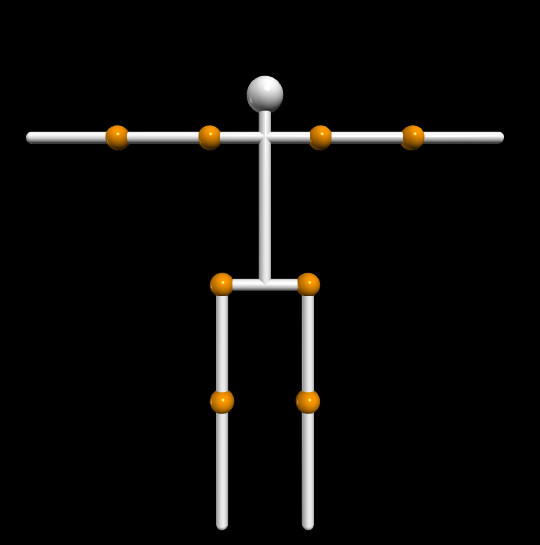
\includegraphics[width=8cm]{fig/testpose1.png}
  \caption{Stick figure to represent a human in pose reconstruction.}
  \label{fig:stickman}
\end{figure}

Taylor also assumes that point correspondences between a scene and its image can be modeled as a scaled orthographic projection. In this model, the image coordinates $(u,v)$ are related to the scene coordinates $(x,y,z)$ by
\begin{align}
  \mqty( u \\ v ) = s \mqty(1 & 0 & 0 \\ 0 & 1 & 0 )\mqty( X \\ Y \\ Z ).
  \label{eq:projection}
\end{align}

This model holds well in pictures with minimal perspective distortion, where the $z$ extent of the subject is small compared to the distance to the camera. By comparing to a more realistic perspective projection model which accounts for the focal length of a simulated camera, Taylor showed that the scaled orthographic projection is sufficiently accurate for most photos of humans. Specifically, he showed that one can expect errors less than 5\% when the camera distance is beyond 5 times the $z$-extent of the subject.

The stick figure has 25 independent degrees of freedom, 4 for each limb, 8 for the torso, and an unknown scale factor $s$. Comparing this to the 24 independent image measurements of the 2D joint locations of the right shoulder, left shoulder, right hip, left hip, right elbow, left elbow, right knee, left knee, right wrist, left wrist, right ankle, and left ankle, we will expect multiple solutions. Taylor chooses the free parameter in the reconstruction to be the scale $s$ and uses geometrical considerations from the scaled orthographic projection to write the reconstruction as a function of $s$.

\begin{figure}[h]
  \centering
  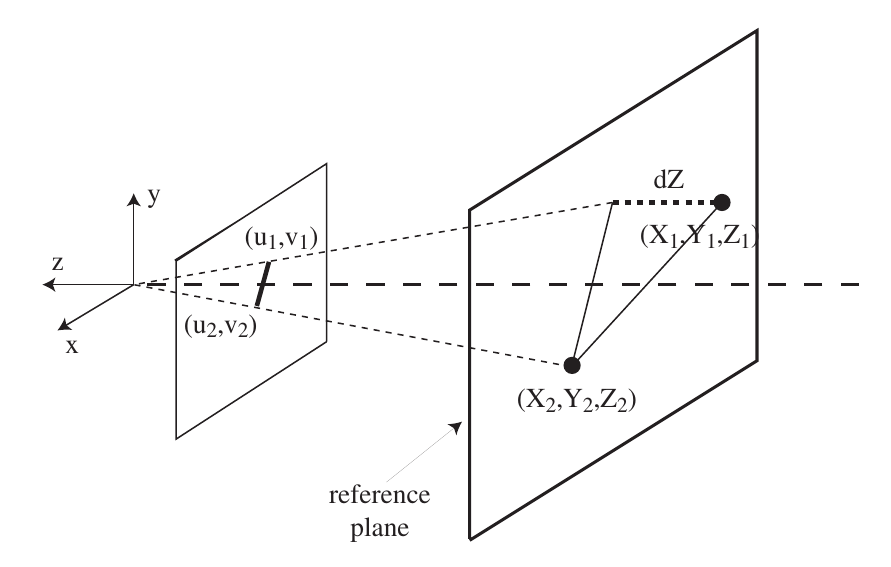
\includegraphics[width=10cm]{fig/projection.png}
  \caption{Figure from Taylor's paper\cite{Taylor} showing the projection of a line segment onto an image under scaled orthographic projection.}
  \label{fig:unproject}
\end{figure}

In Figure \ref{fig:unproject} we depict scaled orthographic projection of a limb of fixed length $l$. Knowing the scale $s$, it is a simple geometric matter to compute the allowed relative depth of the two endpoints $dZ$:

\begin{align}
  l^2 &= \qty(X_1 - X_2)^2 + \qty(Y_1 - Y_2)^2 + (Z_1 - Z_2)^2 \\
  (u_1 - u_2) &=  s(X_1 - X_2) \\
  (v_1 - v_2) &= s(Y_1 - Y_2) \\
  dZ &=  (Z_1 - Z_2) \\
  \Rightarrow dZ &= \pm\sqrt{l^2 - \frac{\qty(u_1 - u_2)^2 + (v_1 - v_2)^2}{s^2}}.
  \label{eq:dZ}
\end{align}

Notice that this equation for $dZ$ constrains the allowable scale $s$ since $dZ$ cannot be complex. Thus, the quantity under the square root must be non-negative, giving the restriction
\begin{align}
  s \geq \frac{\sqrt{\qty(u_1 - u_2)^2 + (v_1 - v_2)^2}}{l}.
  \label{eq:scalecons}
\end{align}
Such a restriction exists for every limb in the stick figure, so the overall scale is has to be at least as large as the largest of the constraints. 

From equation \ref{eq:dZ} we see that the scale determines how slanted a line segment is towards the camera. The larger the scale, the closer the subject is to the image plane. From these considerations, we can develop an intuitive understanding of the scale constraint in equation \ref{eq:scalecons}. A line segment with fixed endpoint projection $(u_1,v_1)$,$(u_2,v_2)$ on the image plane has to become increasingly upright as it is moved away from the camera (hence decreasing scale $s$). However, at one point it will be perpendicular to the $z$ direction, \emph{i.e.} it will be flush with the reference plane. It would no longer be possible to move the segment back further without changing the projection on the image plane, hence setting a minimum scale $s$ corresponding to this maximum distance.

As mentioned in the introduction, in most pictures of humans there will be at least one limb nearly perpendicular to the line of sight. This means that simply using the minimum allowable scale in the 3D reconstruction will give reasonable results for the majority of cases.

Note that in equation \ref{eq:dZ} we do not know the sign of the $Z$ difference in segment endpoints. In a system with multiple segments connected by joints at their endpoints, like the one shown in Figure \ref{fig:unprojectmultiple}, this ambiguity implies $2^N$ allowed reconstructions for fixed scale $s$, where $N$ is the number of limbs. In the stick figure we use, this corresponds to $2^{11} = 2048$ possible reconstructions. However, by specifying the relative ordering of the endpoints for every limb, a unique solution is obtained.

\begin{figure}[h]
  \centering
  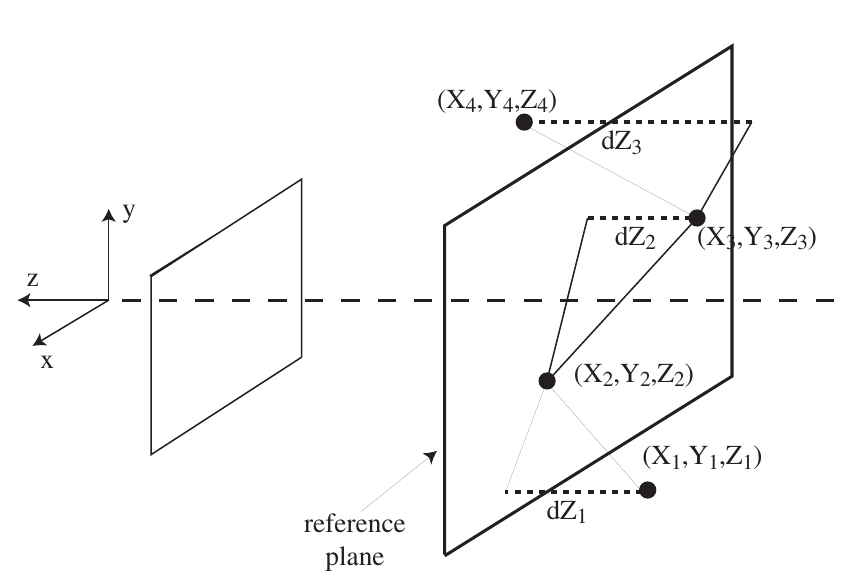
\includegraphics[width=10cm]{fig/projection2.png}
  \caption{A figure from Taylor's paper\cite{Taylor} showing the projection of an articulated object onto an image under scaled orthographic projection}
  \label{fig:unprojectmultiple}
\end{figure}

For this project I implemented Taylor's method (Listing \ref{pointstopos} and designed a graphical user interface for selecting joints on an image and indicating which ends of limbs are closer using \code{tkinter}. An example of it in action is shown in Figure \ref{fig:boltgui}. The code for the GUI is in Listing \ref{gui} and the 3D rendering is done using \code{vpython}, with the script in Listing \ref{renderstick}. Initially I used \code{matplotlib} for 3D rendering, with prototype code shown in Listing \ref{drawstick}, but \code{matplotlib} is not well suited for 3D plotting and does not properly perform depth ordering so the resulting figures are harder to interpret.

\begin{figure}[h]
  \centering
  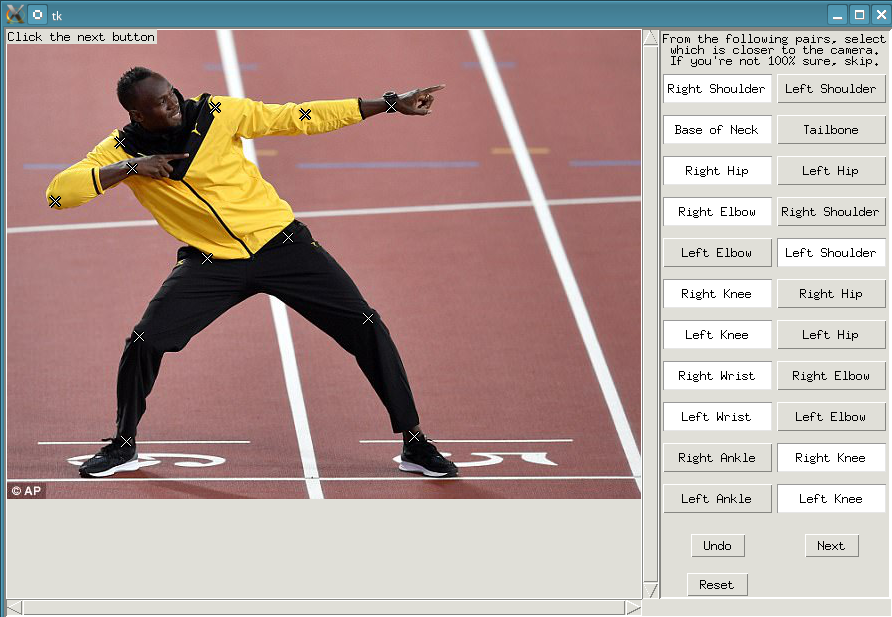
\includegraphics[height=7cm]{fig/boltgui.png}
  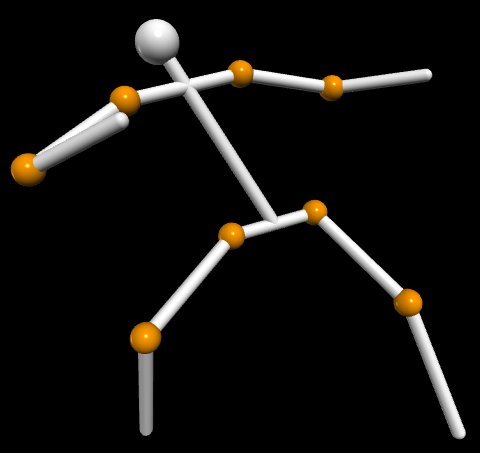
\includegraphics[height=7cm]{fig/boltrecons.png} \\
  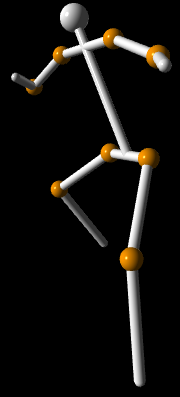
\includegraphics[height=7cm]{fig/boltrecons2.png}
  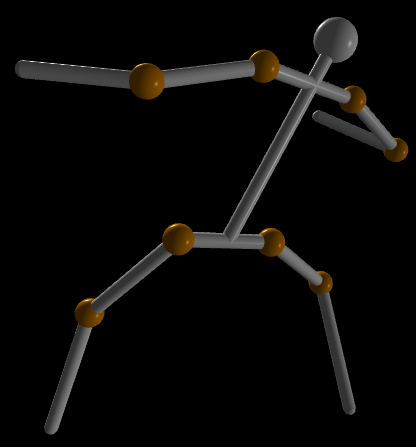
\includegraphics[height=7cm]{fig/boltrecons3.png}
  \caption{My implementation of Taylor's method applied to the well-known pose of Usain Bolt. In the graphical interface the user is prompted to select the positions of joints on the image, and to select which of the displayed joints are closer to the camera.}
  \label{fig:boltgui}
\end{figure}

\subsection{My Method for Incorporating Joint Position Uncertainty and Optimizing in-plane Limbs}

While Taylor's approach usually works well if joint positions and limb endpoint orderings are known exactly, if either of these is difficult to determine, the reconstruction can be very wrong. As shown in Figure \ref{fig:jordangui}, the difficulty in intuiting the hip joint locations and endpoint ordering results in a poor reconstruction. Furthermore, the difficulties are compounded by the fact that the subject likely has different limb proportions than the average human.

\begin{figure}[h]
  \centering
  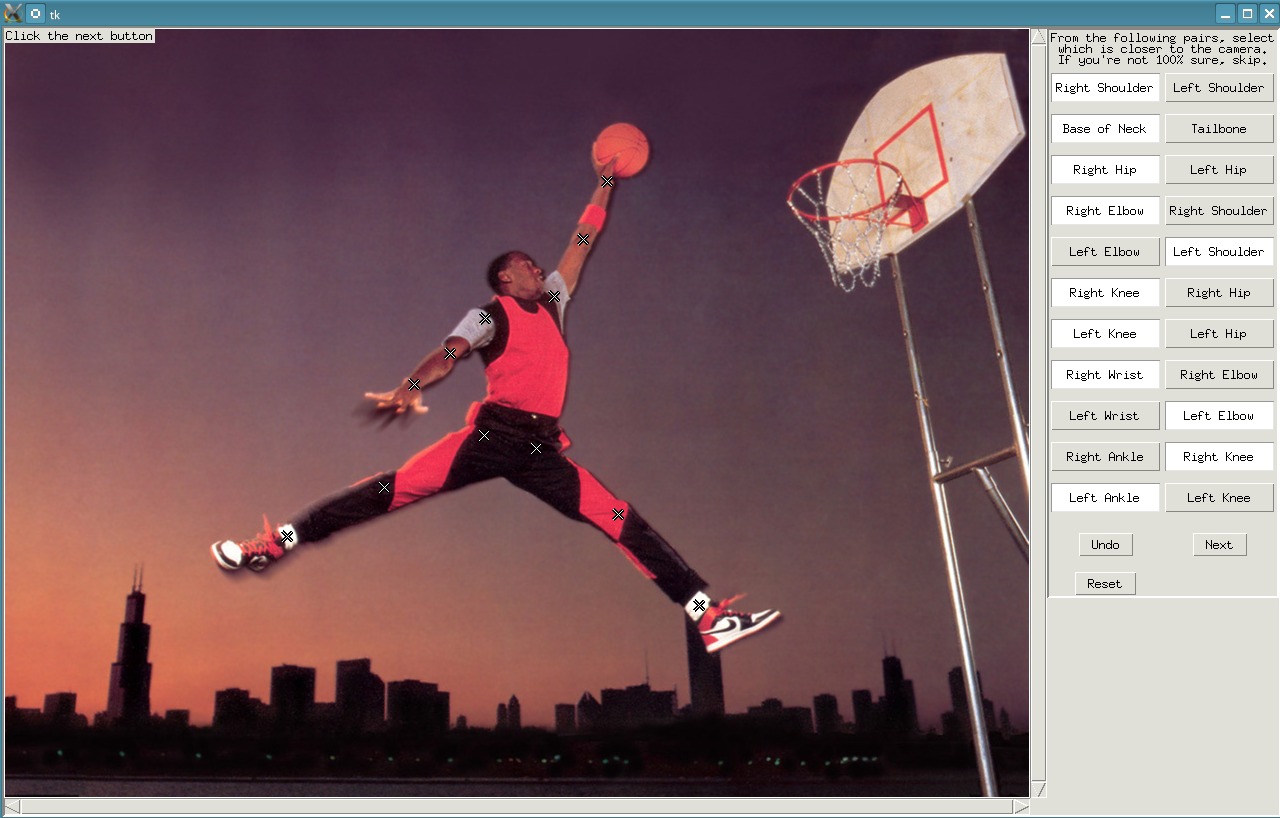
\includegraphics[width=12cm]{fig/jordangui.png}
  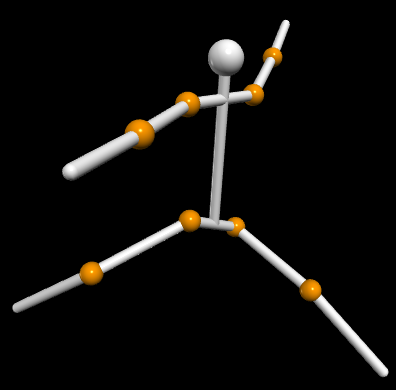
\includegraphics[height=7cm]{fig/jordanrecons.png}
  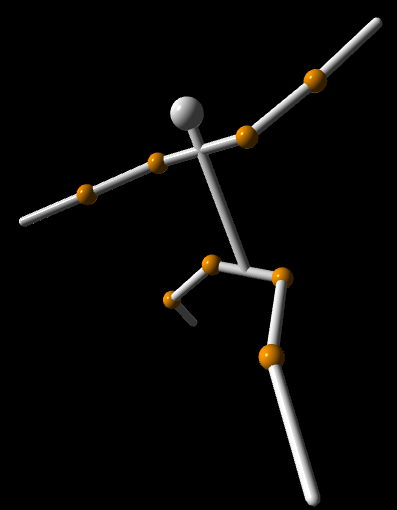
\includegraphics[height=7cm]{fig/jordanrecons2.png}
  \caption{Taylor's method performing poorly on an iconic Michael Jordan pose where many limbs are parallel to the image plane. From the original image, we intuitively know that the legs and left arm are all nearly straight, but there is no way to convey this information to Taylor's algorithm.}
  \label{fig:jordangui}
\end{figure}

I discovered that the two aforementioned difficulties for Taylor's method can actually be turned into a strength. Not knowing which end of a limb is closer to the camera contains important information in itself; namely, it tells us that a limb is very nearly perpendicular to the line of sight. Combined with a user conveying a range of uncertainty in 2D joint positions, it is possible to establish a constrained optimization problem.

\subsubsection{Mathematical Formulation}
First we introduce some mathematical notation for the problem to aid in discussing the proposed optimization. Suppose we have joint index $j \in \qty{1,2,\ldots,12} = \mathbb{J} $ where each index $j$ corresponds to

\begin{center}
  \begin{tabular}{cc}
    \toprule[1.5pt]
    joint index $j$ & joint \\
    \midrule[1pt]
    1 & right shoulder \\
    2 & left shoulder \\
    3 & right hip \\
    4 & left hip \\
    5 & right elbow \\
    6 & left elbow \\
    7 & right knee \\
    8 & left knee \\
    9 & right wrist \\
    10 & left wrist \\
    11 & right ankle \\
    12 & left ankle \\
    \bottomrule[1.5pt]
  \end{tabular}
\end{center}
 in order. Let $\vb{U}$ be a vector constructed from the image points $(u,v)$ of the joints in order, \emph{i.e.} $\vb{U} = (u_1,v_1,u_2,v_2,\ldots,u_{12},v_{12})$, and $\vb{P}$ be a vector of the actual 3D joint positions $(X,Y,Z)$, also assembled in order. Let $\vb{o}$ be a ``relative ordering'' array consisting of $-1$ and $+1$s with each element depending on the answer to which neighboring joint is closer to the camera in the following pairwise comparisons: 
\begin{center}
  \begin{tabular}{cc}
    \toprule[1.5pt]
    ``limb'' index $\ell$ & ``limb'' \\
    \midrule[1pt]
    1 & (right shoulder, left shoulder) \\
    2 & (collarbone, tailbone) \\
    3 & (right hip, left hip) \\
    4 & (right elbow, right shoulder) \\
    5 & (left elbow, left shoulder) \\
    6 & (right knee, right hip) \\
    7 & (left knee, left hip) \\
    8 & (right wrist, right elbow) \\
    9 & (left wrist, left elbow) \\
    10 & (right ankle, right knee) \\
    11 & (left ankle, left knee) \\
    \bottomrule[1.5pt]
  \end{tabular}
\end{center}
 
Let the aforementioned pairwise comparisons be indexed by $\ell$ for future reference. Taylor's reconstruction algorithm $\mathcal{T}$ is then a (single-valued) function which takes $\vb{U}$ and $\vb{o}$ and returns $\vb{P}$,
\begin{align}
  \mathcal{T}(\vb{U},\vb{o}) = \vb{P},
  \label{eq:Taylor}
\end{align}
where we assume that the scale parameter $s$ which the solution also depends on is always chosen to be the minimum allowed in order to make the function single-valued. While any vector $\vb{U} \in \mathbb{R}^{24}$ is allowed, note that $\vb{P} \in \mathbb{R}^{36}$ is constrained by the fact that neighboring joints have relative distances fixed by limb lengths. This constraint does not have to be explicitly imposed since it is true by construction in the Taylor algorithm.

My proposed method allows for radii of uncertainty $r$ to be passed alongside each joint's image position, implicitly indicating that a given joint's true image position $(u,v)$ is likely within a circle of radius $r$ from the user-supplied joint image position $(u_0,v_0)$, \emph{i.e.} $\sqrt{(u-u_0)^2 + (u-v_0)^2} \leq r$. Let the array $\vb{r}$ be have elements $r$ for each joint in order. Furthermore, define a new augmented relative ordering array $\vb{o_a}$ which follows the same rules as the relative ordering array $\vb{o}$ except an element is allowed to be $0$ when the $z$-ordering endpoints of the corresponding limb is uncertain (and hence the limb is parallel to the image plane).

\subsubsection{Optimization Problem Description}

Now, given the initial guess vector of joint locations $\vb{U}_0$, There is a set of possible image point functions $\mathbb{U}_{\vb{U}_0,\vb{r}} \subset \mathbb{R}^{24}$ where any $\vb{U} \in \mathbb{U}_{\vb{U}_0,\vb{r}}$ has to obey 
\begin{align}
  \norm{U_j - U_{0j}}_2 \leq r_j,
  \label{eq:ineqcons}
\end{align}
for all $j \in \mathbb{J}$, where $U_j$ is the image position $(u_j,v_j)$ of joint $j$. This space $\mathbb{U}_{\vb{U}_0,\vb{r}}$ describes the domain of a constrained optimization function.

The objective function in this minimization problem penalizes nonzero $dZ$ for limbs whose endpoints are said to be nearly in plane, \emph{i.e.} where $o_{a,\ell} = 0$, with ``limb'' index $\ell$ defined earlier. Let the function $dZ(\ell,\vb{P})$ be defined to take a limb index $\ell$ and 3D joint positions $\vb{P}$ and return the difference in $z$ coordinate of the two endpoints of limb $\ell$. For the ``limb'' $\ell = 2$ with endpoints being the collarbone center and tailbone, note that these points are fully determined by the shoulder and hip positions so $dZ(2,\vb{P})$ is still well defined.

So, formally our objective function $f_{\vb{o}}$ is given by
\begin{align}
  f_{\vb{o}}(\vb{U}) &= \sum_{\qty{\ell | o_{a,\ell} = 0}} dZ^2[\ell,\mathcal{T}(\vb{U},\vb{o})]
  \label{eq:objectivefn}
\end{align}
where $\mathcal{T}$ is the Taylor algorithm for turning image points $\vb{U}$ into 3D positions $\vb{P}$. Notice that the objective function has a subscript $\vb{o}$ which is to indicate that it depends on a relative ordering array $\vb{o}$, as required by the Taylor algorithm. For a given augmented relative ordering array $\vb{o_a}$, there are still $2^m$ possible relative ordering arrays $\vb{o}$ where $m$ is the number of zeros in $\vb{o_a}$. This reflects the fact that for limbs very nearly parallel to the image plane, there is still one endpoint that is closer than another. We simply expand our minimization problem by computing $\displaystyle\min_{U \in \mathbb{U}_{\vb{U}_0,\vb{r}}}f_{\vb{o}}(\vb{U})$ for all $\vb{o}$ compatible with $\vb{o_a}$, and picking the configuration with the smallest penalty of all of them. To be clear, a relative ordering $\vb{o}$ is compatible with $\vb{o_a}$ if its elements match all the nonzero elements of $\vb{o_a}$.

So, writing the optimization problem down completely,

\begin{align}
  \vb{U}_{\trm{min}} = \argmin_{U \in \mathbb{U}_{\vb{U}_0,\vb{r}}} f_{\vb{o}_{\trm{min}}}(U), \qq{where} \vb{o}_{\trm{min}} = \argmin_{\vb{o} \trm{ compatible } \vb{o_a}} \qty[ \min_{U \in \mathbb{U}_{\vb{U}_0,\vb{r}}} f_{\vb{o}}(U)]
  \label{eq:optformal}
\end{align}

To solve this optimization problem, I used the \code{scipy.optimize.minimize} implementation of the COBYLA (constrained optimization by linear approximation) method for constrained nonlinear optimization. COBYLA does not need derivative information. It iteratively approaches a solution using linear approximations of the objective function, solving them on a simplex. This method works well with the inequality constraints we have in this problem, equation \ref{eq:ineqcons}. I chose to use this method since local minima of the objective function appear to be adequate for our purposes, and global minimization would take too long with the high dimensionality of the problem. 

\subsubsection{Taylor Method with Joint Uncertainty and In-Plane Optimization}

Now we can write down my modification to the Taylor method in terms of the previous mathematical quantities. Given an initial image position guess vector $\vb{U}_0$, uncertainty array $\vb{r}$, and augmented relative ordering array $\vb{o_a}$, the reconstructed 3D positions are given by
\begin{align}
  \mathcal{F}(\vb{U}_0,\vb{r},\vb{o_a}) &= \mathcal{T}\qty(\vb{U}_{\trm{min}},\vb{o}_{\trm{min}}).
  \label{eq:mymethod}
\end{align}
Note that if the augmented relative ordering array contains no zero elements, then it is simply a relative ordering array $\vb{o}$ and my method reduces to the Taylor method.

The code for the optimization problem and for my improvement to the Taylor algorithm is shown in Listing \ref{optimizepoints}.

The interface I created allows users to specify a radius of uncertainty for each joint by clicking and dragging to create a circle. As a demonstration of my approach, see Figure \ref{fig:myjordan}. Notice that it much better captures the subject's pose. Remember that this is accomplished by perturbing the joint positions \emph{and} by choosing the optimal relative ordering array for ordering limb endpoints for limbs that are very nearly parallel to the image plane.

\begin{figure}[h]
  \centering
  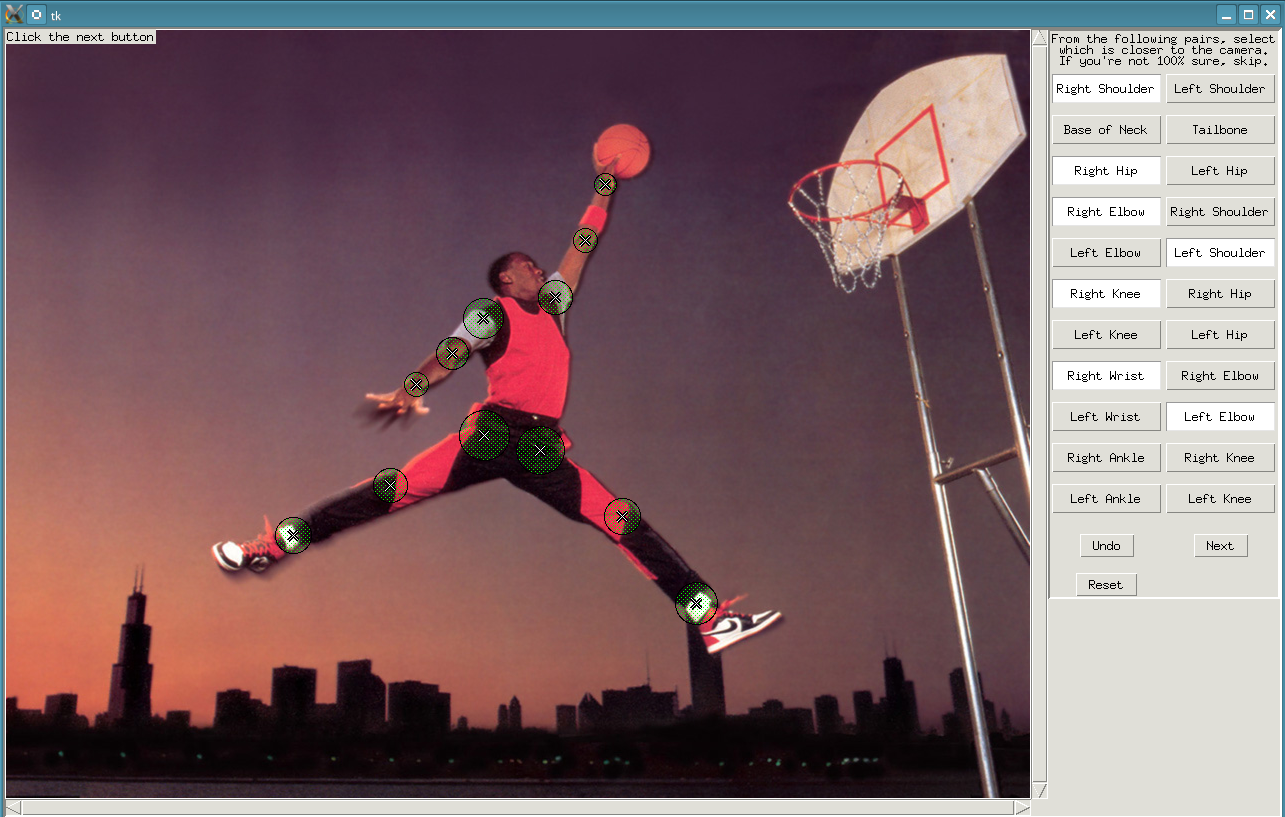
\includegraphics[width=12cm]{fig/myjordan.png}
  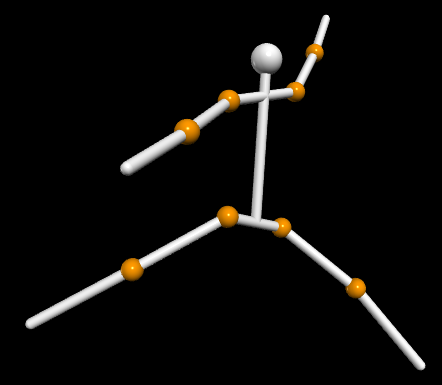
\includegraphics[height=7cm]{fig/myjordanrecons.png}
  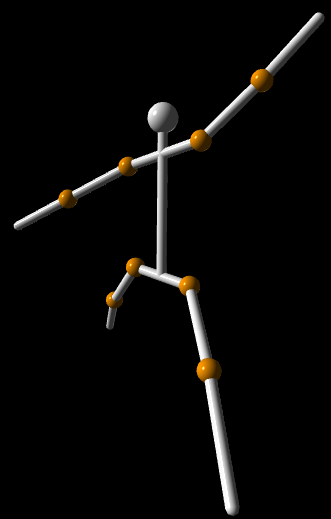
\includegraphics[height=7cm]{fig/myjordanrecons2.png}
  \caption{My improvement to Taylor's method by allowing uncertainties in joint positions, as well as optimization of in-plane limbs. Compare this reconstruction to one with the Taylor method shown in Figure \ref{fig:jordangui}.}
  \label{fig:myjordan}
\end{figure}

\newpage
\section{Quantitative Comparison of Improved Method to the Original Taylor Method}

In order to quantitatively compare my modified Taylor method to the original Taylor method, we need a ground truth that we can compare to. One way to achieve this is by posing a stick figure in 3D and computing the scaled orthographic projection as a forward problem. In order to make the performance test objective, I add Gaussian noise to the 2D joint image positions to simulate a user not being able to exactly identify where a skeletal joint is located in the bulk of a subject's body. This is all Taylor's method gets in terms of information, while my method additionally receives a reasonable estimate of the standard deviation of the Gaussian noise to represent the user's ability to specify their uncertainty in their selected joint location. Both methods then reconstruct the 3D joint position information, which is then compared to the known ground truth.

\subsection{Generating Simulated Human Positions and Image Data}

In order to produce a valid set of 3D joint positions $\vb{P}$ which obey the limb length constraints, it is easiest to use a coordinate system where this constraint is built in. I chose to have limb directions be specified by two local angles $\theta,\phi$ each, with the head setting the initial position for the body. These rotations are all specified relative to a default rotation vector defined locally for each joint. Then, $\theta$ describes the rotation in the direction of the rotation vector (counter-clockwise), while $\phi$ angles the rotation vector itself in the $z$ direction. To obtain the Cartesian coordinates $\vb{P}$, the default stick figure configuration shown in Figure \ref{fig:stickman} has its limb vectors rotated by rotation matrices specified by these $\theta$ and $\phi$. This is performed numerically using the Euler-Rodrigues formula to compute a rotation matrix which rotates by $\theta$ about the rotation vector which has been tilted towards or away from $\vu{z}$ by $\phi$. The code for this can be found in Listing \ref{rotmat}. In order obtain the proper direction for the extremal limb vectors, the rotation matrices for all the limbs connecting it back to the head are applied. For example, for the right forearm, its limb vector is rotated by the rotation matrix at the right elbow, then by the rotation matrix of the right shoulder, then by the rotation matrix of the right collarbone, then finally by the rotation matrix of the head. Once all the limb vectors are pointing the specified directions, a subset can simply be added in sequence to find a given joint position. The code for computing $\vb{P}$ from the local angles is in Listing \ref{angletopos}.

\subsubsection{Computing the Scaled Orthographic Projection}

The scaled orthographic projection is simply calculated from equation \ref{eq:projection}, where we are free to choose a scale. We pick $s = 1$ since it does not matter for the forward problem; it just sets the ``size'' of the image. The relative 2D joint positions of the projection will be the same either way. The code for this part is in Listing \ref{postopoints}. After the projection is computed, for the purposes of the performance test we add some 2D Gaussian noise with a standard deviation of $\sigma = 0.05 \times \trm{height}$ in each direction, to the position of each limb. For a person of height $178\uu{cm}$, this is an uncertainty of $8.9\uu{cm}$ in the limb position, which is not too unreasonable for the shoulder and hip location uncertainty in a bulky human. I applied the same amount of uncertainty to every limb for simplicity, but it would be more realistic to have smaller uncertainties for elbow, wrist, and ankle joints due to their smaller size.

\subsection{Poses}

For the following performance test, I created a few test poses that have a certain number of nearly in-plane limbs (limbs perpendicular to line of sight). 

\subsubsection{Test Pose 1, All Limbs Perpendicular}

The code to generate this pose is in Listing \ref{testpose1}. 

\begin{center}
  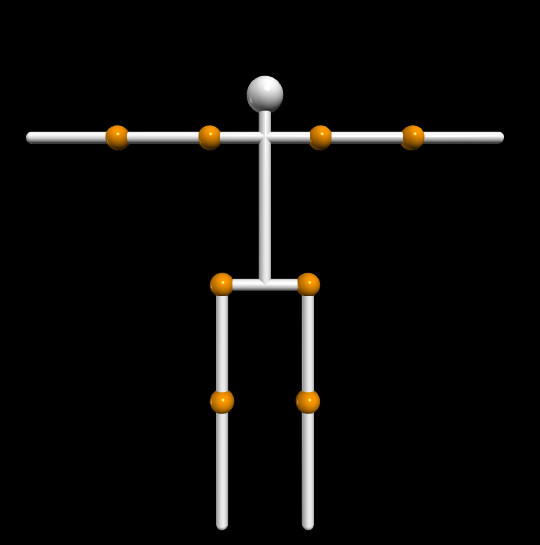
\includegraphics[height=6cm]{fig/testpose1.png}
  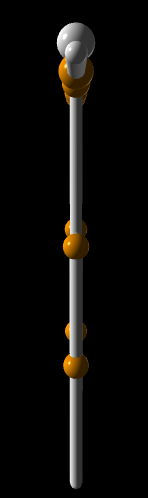
\includegraphics[height=6cm]{fig/testposeside1.png}
\end{center}

In this very simple pose, all limbs are parallel to the image plane.

\subsubsection{Test Pose 2: Four Limbs Perpendicular}

The code to generate this pose is in Listing \ref{testpose2}. 

\begin{center}
  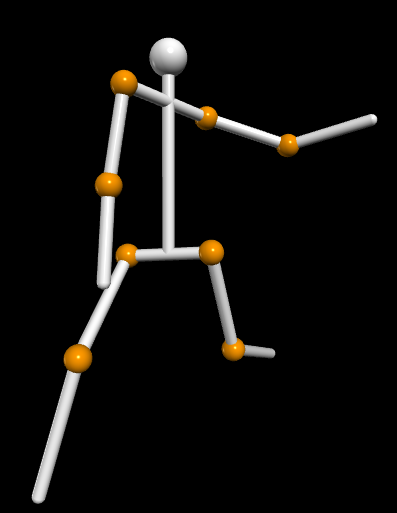
\includegraphics[height=6cm]{fig/testpose2.png}
  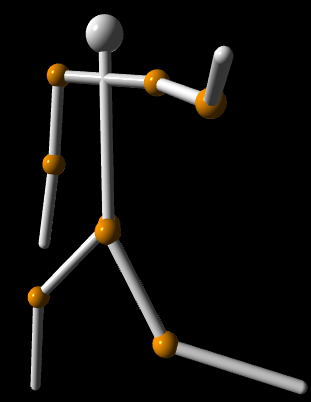
\includegraphics[height=6cm]{fig/testposeside2.png}
\end{center}

In this pose, the right upper arm, right lower arm, hips, and right foreleg are nearly parallel to the image plane.

\subsubsection{Test Pose 3: Two Limbs Perpendicular}

The code to generate this pose is in Listing \ref{testpose3}. 

\begin{center}
  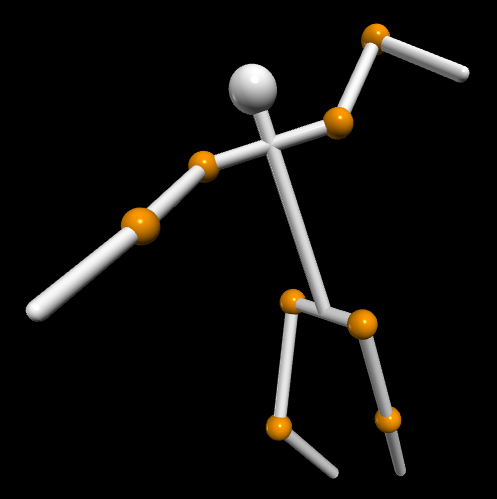
\includegraphics[height=6cm]{fig/testpose3.png}
  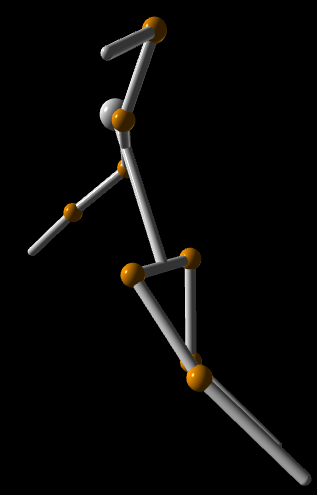
\includegraphics[height=6cm]{fig/testposeside3.png}
\end{center}

In this pose, the shoulders and the right thigh are nearly parallel to the image plane.

\subsubsection{Test Pose 4: One Limbs Perpendicular}

The code to generate this pose is in Listing \ref{testpose4}. 

\begin{center}
  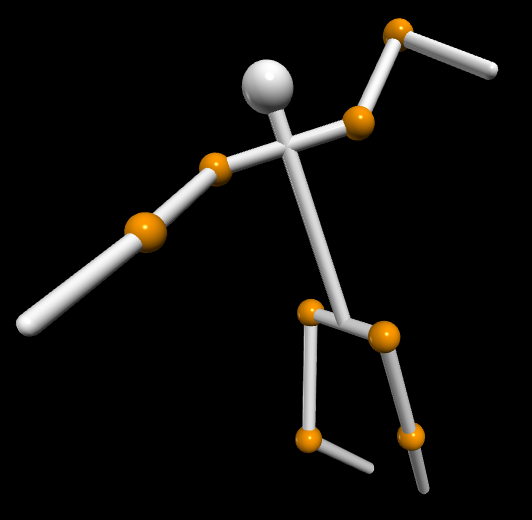
\includegraphics[height=6cm]{fig/testpose4.png}
  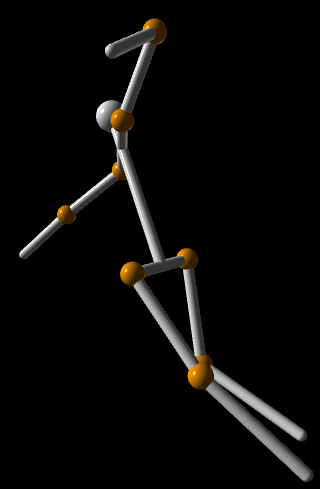
\includegraphics[height=6cm]{fig/testposeside4.png}
\end{center}

This pose is a slight modification to Test Pose 3, where I moved the right thigh back a bit more so that only the shoulders are nearly parallel to the image plane.

\subsection{Pose Reconstruction Error}

In order to compare the methods, I needed a definition of error in the 3D reconstruction. A natural definition for this quantity would penalize for the distance by which each joint position differs from the corresponding true position. However, we do not concern ourselves determining the size of the reconstructed 3D stick figure, as this overall scaling factor does not change the pose. To remove penalties associated with getting this factor wrong, the error function I use contains an optimization problem as well. Given 3D joint positions $\vb{P}$ and a reference $\vb{P}_0$, first I subtract away the average joint position of both to set the center of mass of the points at the origin, and then I allow $\vb{P}$ to be rescaled by a factor $\alpha$. The error as a function of rescaling parameter $\alpha$ is given by
\begin{align}
  E(\alpha,\vb{P},\vb{P}_0) &= \frac{1}{N} \sum_{j\in \mathbb{J}} \norm{\alpha\vb{P}_j - \vb{P}_{0j}}_2
  \label{eq:erroralpha}
\end{align}
where $N = 12$ is the number of joints. This has the interpretation of being the average joint distance away from the reference joint positions. Now, in order to remove the effect of an overall scaling factor $\alpha$, I define the error to be
\begin{align}
  E(\vb{P},\vb{P}_0) \equiv \min_{\alpha \in \mathbb{R}} E\qty(\alpha,\vb{P},\vb{P}_0).
  \label{eq:error}
\end{align}
To solve this minimization problem I use the \code{scipy.optimize.minimize} implementation of BFGS, which works well in this problem since $E(\alpha,\vb{P},\vb{P}_0)$ is coercive, and a smooth function of $\alpha$. The fact that it is coercive also guarantees the existence of a global minimum, so our error function is well defined. I have not ensured that all local minima are global minima for this function, so in principle it would be better to use a global minimization routine. However, the minimization is given $\alpha_0 = 1$ as a starting value, and $\vb{P}_j$ is expected to be very close to the right scale to start with anyways. Empirically I found that the optimal $\alpha$ are always very close to $1$, so we would not expect the error to be significantly different even if there happened to be a local minimum that is slightly larger than the global minimum, as it would have been nearby anyways.


\subsection{Results}

For each of the test poses presented, I generated a set of 10 noisy 2D joint positions which were then given to Taylor's method and my modification to the method. The error definition given in \ref{eq:error} is divided by the height of the stick figure to normalize the distance. This results in an error that can be interpreted as the average distance of a reconstructed joint to the true joint position, relative to the height of the human. Then I computed the average errors from the 10 runs for each test pose and their standard deviations. This information is shown in Figure \ref{fig:performance}.

\begin{figure}[h]
  \centering
  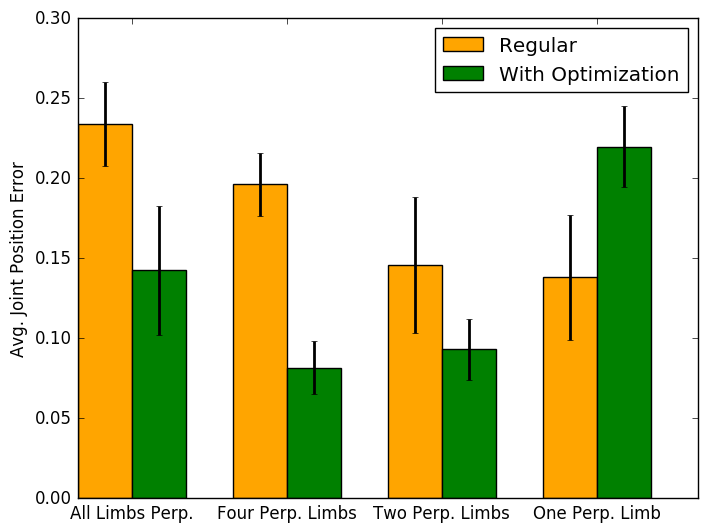
\includegraphics[width=11cm]{fig/performance.png}
  \caption{The average joint position error is measured relative to the height of the original stick figure. The bars labeled ``Regular'' refer to the Taylor method, while the bars labeled ``With Optimization'' incorporate my modification. Notice that when there is more than one limb perpendicular to the line of sight (parallel to the image plane), my method outperforms Taylor's algorithm.}
  \label{fig:performance}
\end{figure}

  The results show that when more than one limb is parallel to the image plane, my method is a significant improvement to the Taylor approach alone. Furthermore, note that in the case where two or four limbs are parallel to the image plane, the average 3D joint position error is comparable to $\sigma\sqrt{8/\pi} = 0.05\sqrt{8/\pi} \approx 0.079$, which is the expected distance a joint would be from the ideal position if the standard deviation $\sigma = 0.05$ we applied to each of the 2D directions were applied to all three directions. This follows from the fact that the expected distance of three independent normally distributed variables of standard deviation $\sigma$ is given by the mean of the $\chi_3$ distribution, $\sigma\sqrt{8/\pi}$.

When there is only one limb parallel to the image plane, my method performs worse than the Taylor method. This could be due to the optimization sacrificing the positions of other joints in order to meet the one constraint. This potentially improves the joint positions on both sides of the one limb whose $dZ$ it tries to optimize, but since the optimization does not penalize motion of the other joint positions, it can result in a worse overall configuration. However, note that these results were only done for a single test pose, Test Pose 4, and it is possible that there are other poses with only one limb parallel to the image plane where my method can outperform the Taylor method. A more thorough investigation would need to randomly sample poses.

The code for these performance tests is shown in Listing \ref{performancetest}.

\section{Qualitative Performance Comparison}

In the following examples, my method performs noticeably better, where our intuition regarding the pose is sufficient to be the judge. Each of these tests was performed on the first try without any tweaking whatsoever.

\subsection{Taylor Method}
\begin{center}
  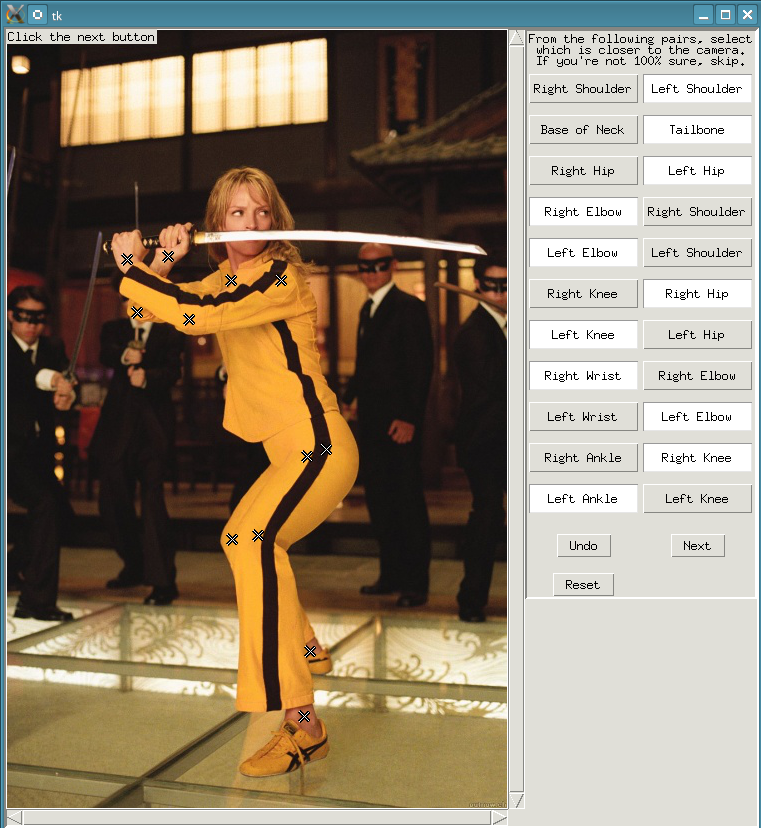
\includegraphics[height=7cm]{fig/killbill.png}
  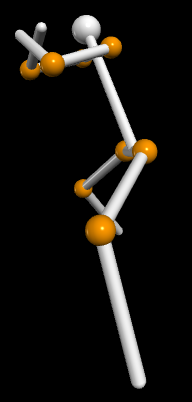
\includegraphics[height=7cm]{fig/killbillrecons.png}
  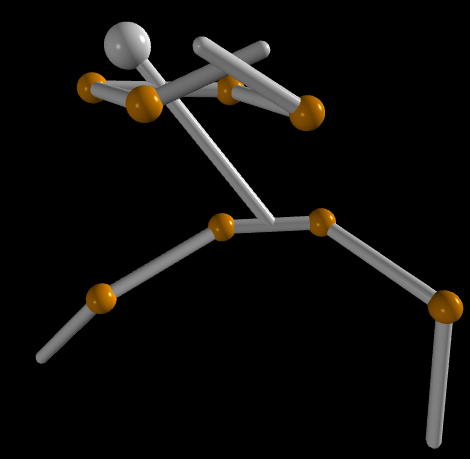
\includegraphics[height=7cm]{fig/killbillrecons2.png}
\end{center}

\subsection{My Method}
\begin{center}
  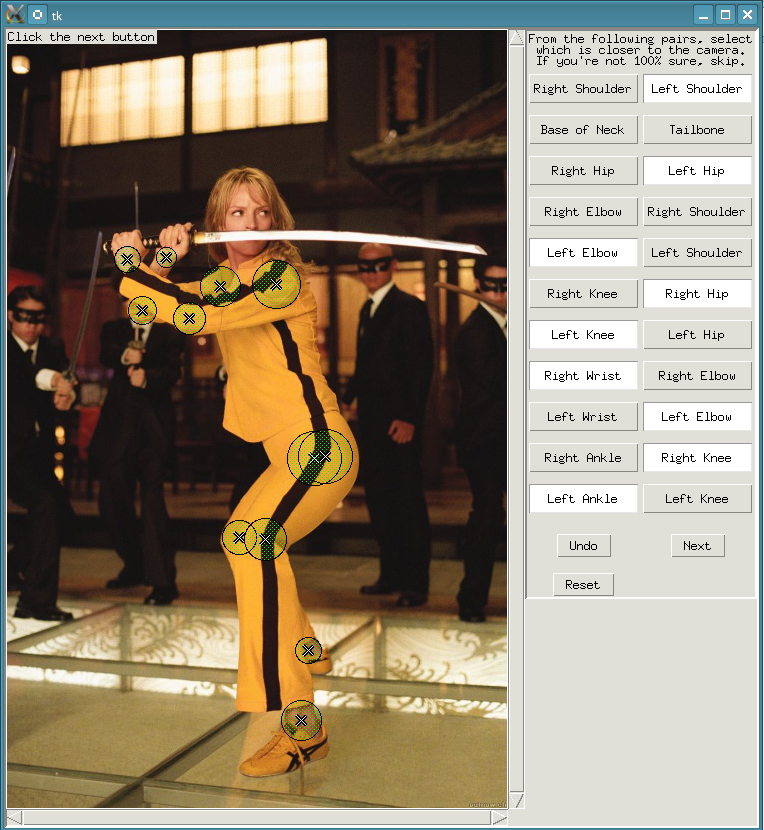
\includegraphics[height=9cm]{fig/mykillbill.png}
  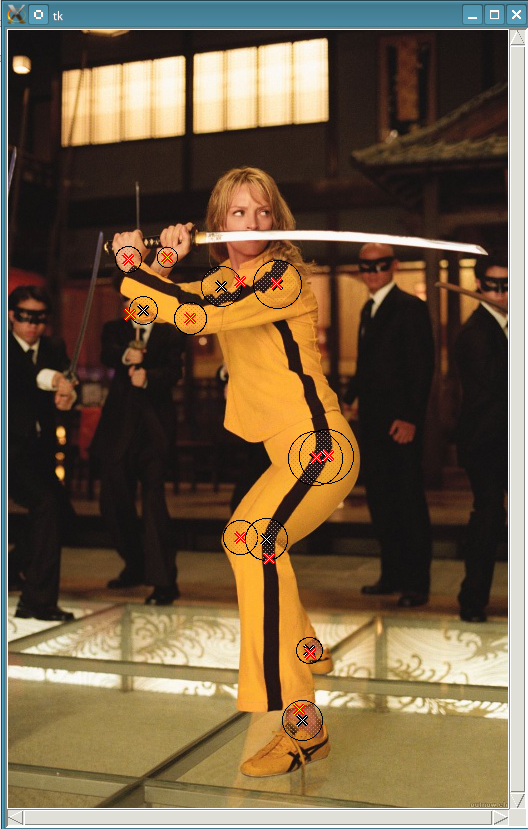
\includegraphics[height=9cm]{fig/mykillbillopt.png} \\
  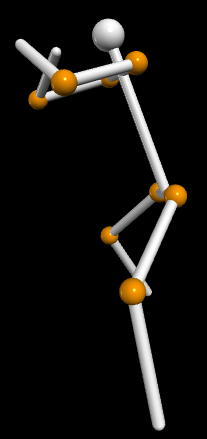
\includegraphics[height=8cm]{fig/mykillbillrecons.png}
  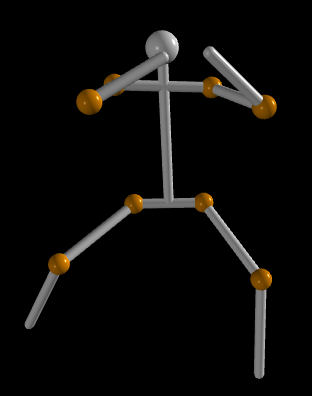
\includegraphics[height=8cm]{fig/mykillbillrecons2.png}
\end{center}

\subsection{Taylor Method}
\begin{center}
  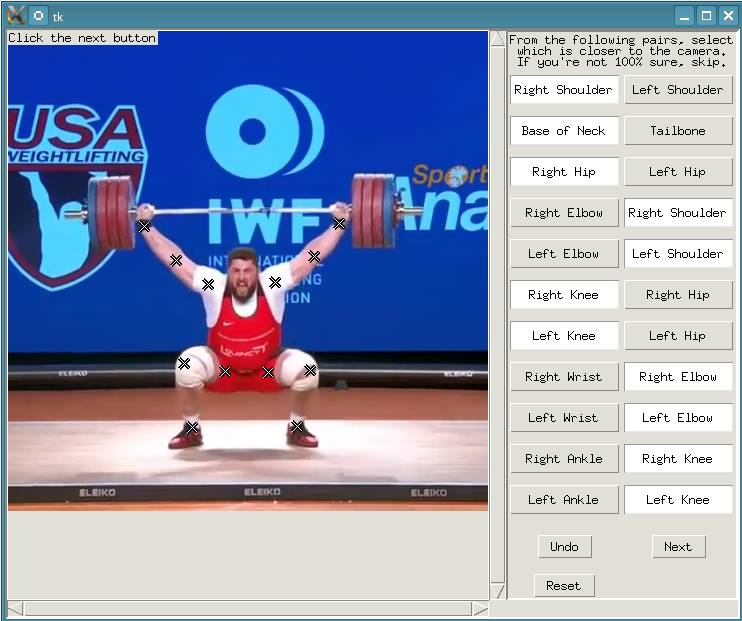
\includegraphics[height=7cm]{fig/jerk.png}
  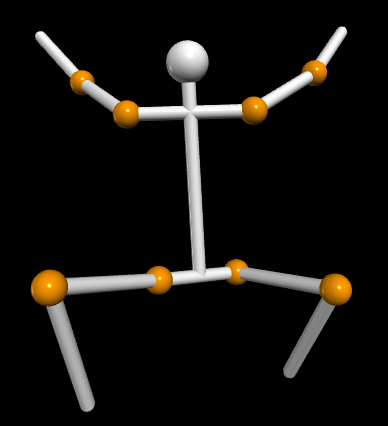
\includegraphics[height=7cm]{fig/jerkrecons.png}
  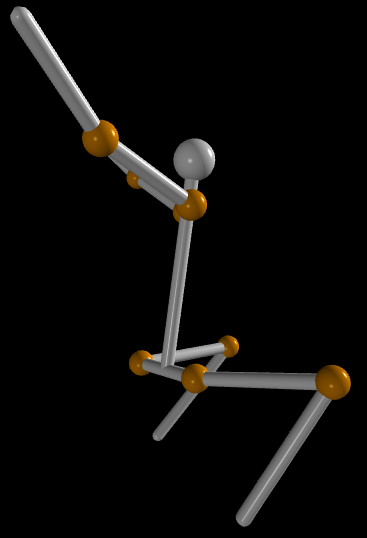
\includegraphics[height=7cm]{fig/jerkrecons2.png}
\end{center}

\subsection{My Method}
\begin{center}
  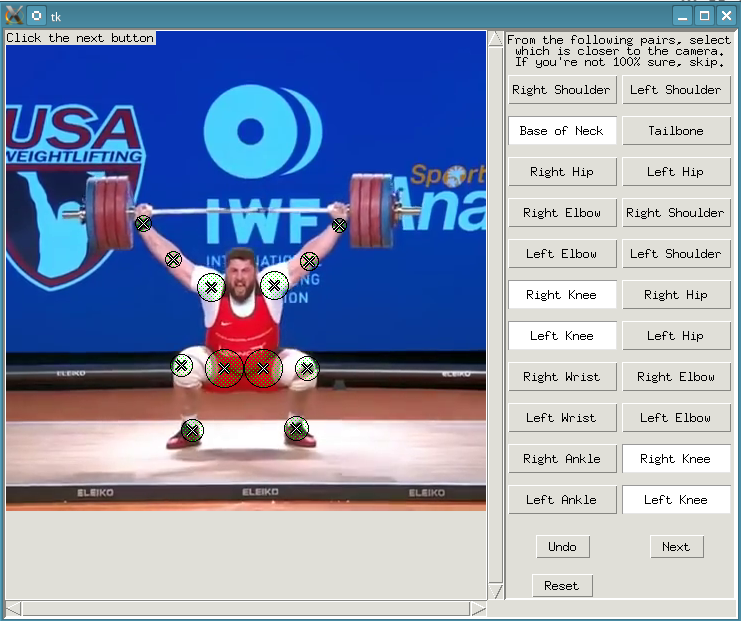
\includegraphics[height=8cm]{fig/myjerk.png}
  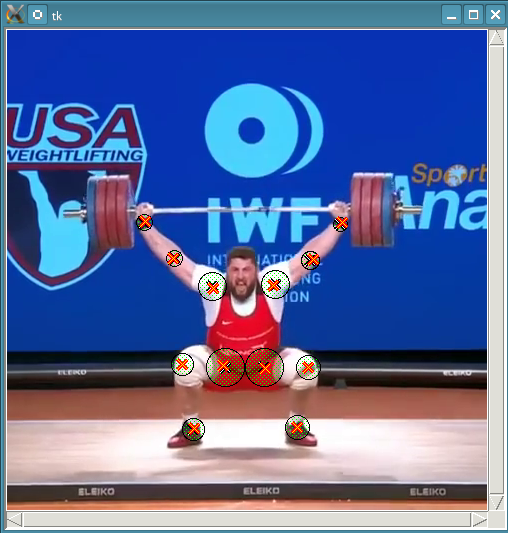
\includegraphics[height=8cm]{fig/myjerkopt.png} \\
  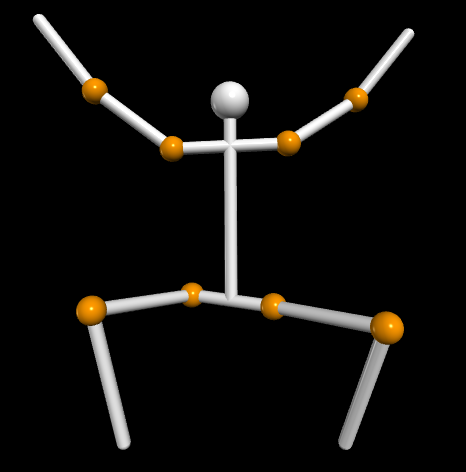
\includegraphics[height=8cm]{fig/myjerkrecons.png}
  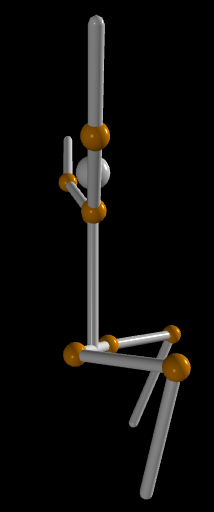
\includegraphics[height=8cm]{fig/myjerkrecons2.png}
\end{center}

\subsection{Taylor Method}
\begin{center}
  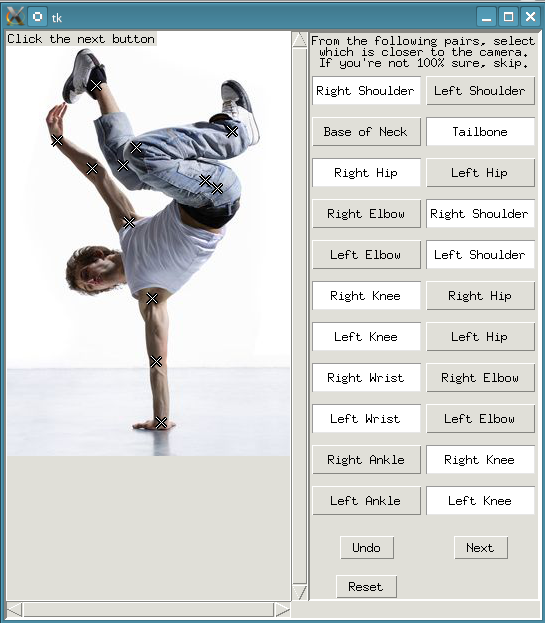
\includegraphics[height=8cm]{fig/breakdance.png}
  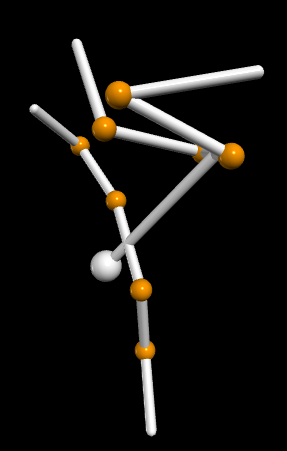
\includegraphics[height=8cm]{fig/breakdancerecons.png}
  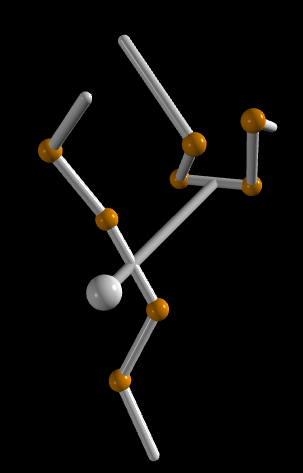
\includegraphics[height=8cm]{fig/breakdancerecons2.png}
\end{center}

\subsection{My Method}
\begin{center}
  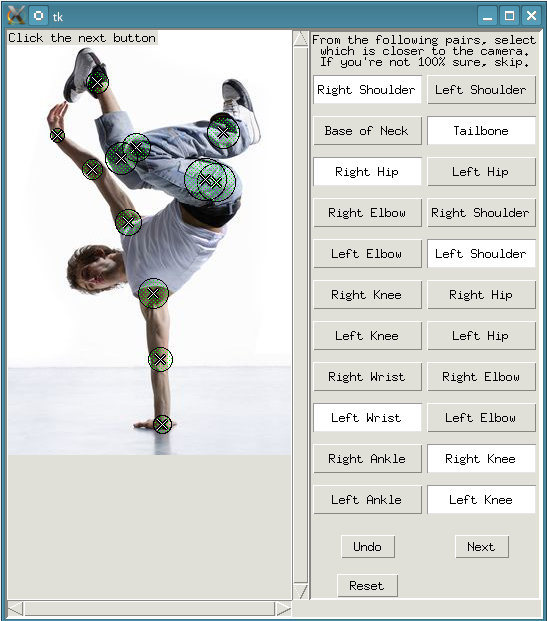
\includegraphics[height=9cm]{fig/mybreakdance.png}
  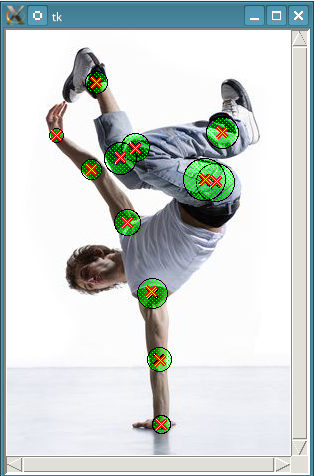
\includegraphics[height=9cm]{fig/mybreakdanceopt.png} \\
  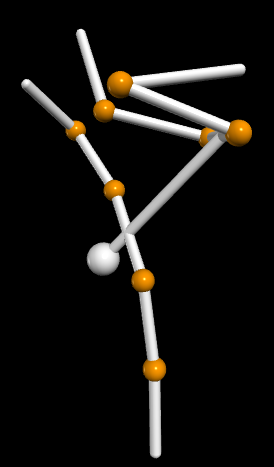
\includegraphics[height=9cm]{fig/mybreakdancerecons.png}
  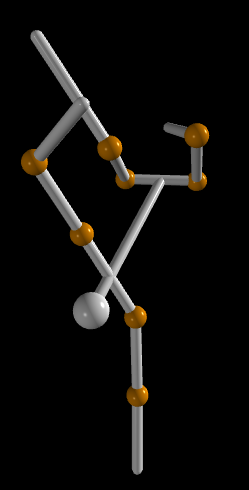
\includegraphics[height=9cm]{fig/mybreakdancerecons2.png}
\end{center}

\section{Conclusions and Outlook}

My method directly addresses the uncertainties that negatively impact the Taylor model, and I show that, surprisingly, these supposed weaknesses can be turned into strengths for the reconstruction process. One possible limitation that I have observed, as shown in the section on Quantitative Results, is that sometimes my method can be worse than the Taylor method when only one limb is perpendicular to the line of sight. If this turns out to generally be the case, we could simply use Taylor's method whenever the number of limbs perpendicular to $\vu{z}$ is one or zero. To better determine quantitative performance, a natural extension to this project would involve automatically generating many more forward problems than the four we have considered here. The results would give a better sense of my method's performance. Furthermore, since the goal of this project is to reconstruct human poses, an even more refined test of performance would consider the likelihoods of given 3D poses. Improved performance on common poses should be more heavily weighted than performance on very uncommon human poses.


For real world application, it would also be useful to pair my method with image recognition software to eliminate manual input of joint positions and orderings. Taylor's method has already been successfully paired with neural networks\cite{Fan} for full automation, so it should be straightforward to implement my approach. If the algorithm for image recognition already has a way to report its uncertainty in a joint location or ordering, this information could be directly passed to the optimization used in the approach presented in this project.

However, this also brings to light a possible limitation to my method, which is shared by the Taylor method. In decoupling the image recognition and the 2D to 3D unprojection, some information is unnecessarily lost. Serra has shown that an approach that closely links the image recognition step with the 3D reconstruction step can outperform two-step approaches when the feature detector in the image recognition step performs poorly\cite{Serra}. Serra's approach uses observations in the image and from trial 3D reconstructions to iteratively approach a self-consistent result. 

My method could also be improved by considering joint angle constraints. There are many limb configurations that are not physiologically possible for the majority of humans, so eliminating this from the search space could result in performance increases. For example, in my method it is possible for the reconstructed pose to have knees bending in the wrong direction, although it is usually not likely if the relative ordering array is correctly set up.

Closely related to monocular pose reconstruction from single images is human motion reconstruction from a monocular video stream. While one could apply single image techniques to each frame of a video stream, much better performance could be obtained from examining frames temporally near the frame in consideration to glean information about the present pose. For example, the scale constraint in equation \ref{eq:scalecons} becomes increasingly restrictive as more frames are analyzed in a video since it becomes almost guaranteed that a limb orients to be perpendicular to the line of sight. Furthermore, temporal information opens up a variety of physically-motivated inference techniques. By constraining motions to be physical, one can again learn a lot about a subject's pose at any given time.

\bibliography{refs}
\bibliographystyle{ieeetr}

  \section{Code}
     \pythonscript{meas}{Relative limb measurements}

     \pythonscript{run}{Script to launch GUI and pose reconstruction}

     \pythonscript{gui}{Tkinter code for generating a GUI for joint selection and ordering}

     \pythonscript{pointstopos}{Taylor method implementation}

     \pythonscript{renderstick}{Vpython code for rendering a stick figure in the determined 3D pose}

     \pythonscript{drawstick}{Prototype code for drawing a 3D stick figure using matplotlib}

     \pythonscript{optimizepoints}{My improvement to the Taylor algorithm for 3D pose reconstruction using optimization}

     \pythonscript{rotmat}{Rotation matrix generated using the Euler-Rodrigues formula}

     \pythonscript{angletopos}{For generating joint positions from local angles}

     \pythonscript{postopoints}{Scaled orthographic projection}

     \pythonscript{testpose1}{Test Pose 1 generator}

     \pythonscript{testpose2}{Test Pose 2 generator}

     \pythonscript{testpose3}{Test Pose 3 generator}
     
     \pythonscript{testpose4}{Test Pose 4 generator}

     \pythonscript{performancetest}{Tests performance of my method against Taylor's for Test Pose 1-4}

     \pythonscript{displaynewpoints}{Launches a tkinter instance to display the 2D image along with the optimized 2D joint locations}




\end{spacing}
\end{document}
